\providecommand{\main}{..}
\documentclass[\main/notes.tex]{subfiles}

\begin{document}
	\ifSubfilesClassLoaded{\setcounter{chapter}{7}}{}
	\addtocontents{toc}{\protect\newpage}
	\chapter{Algorithms}
		\begin{definition}{Algorithm (basic)}
			A step-by-step method for solving a problem, or doing a task. Accepts \concept{input data}, and creates \concept{output data}.
		\end{definition}
		\section{Algorithm Constructs}
			\begin{description}[nosep]
				\item[Sequence] A group of instructions done in order. Can be simple, or contain the other constructs.
				\item[Decision] Performing certain instructions based on a condition.
				\item[Repetition] Repeat the same sequence of instructions multiple times.
			\end{description}
		\section{Algorithm Representation}
			\subsection{Unified Modeling Language (UML)}
				\begin{definition}{Unified Modeling Language (UML)}
					Pictorial representation of an algorithm. Hides detail, shows how the algorithm flows.
					\begin{center}
						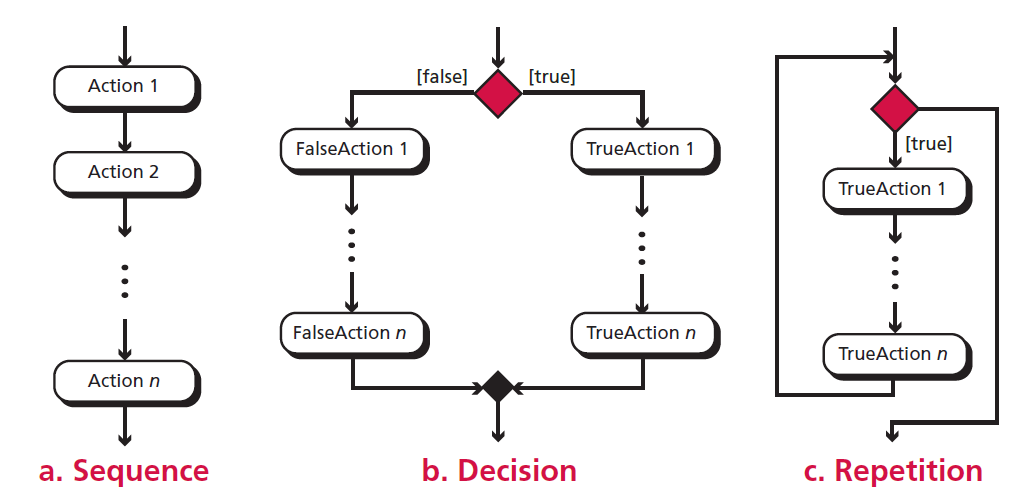
\includegraphics[width=0.8\textwidth]{\main/images/unit08/uml.png}
					\end{center}
				\end{definition}
			\subsection{Psuedocode}
				\begin{definition}{Pseudocode}
					An English-link representation of an algorithm. No standard for how it is written. An example would be:
					\begin{center}
						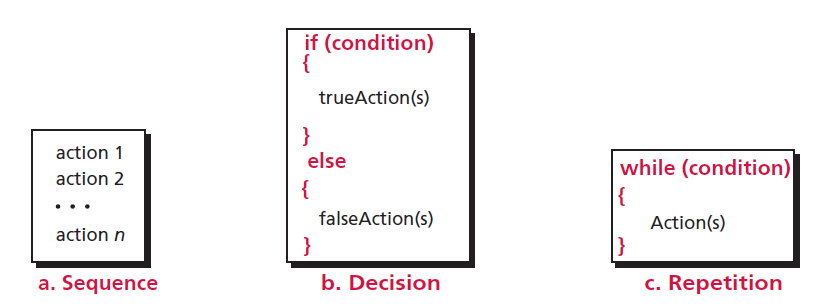
\includegraphics[width=0.8\textwidth]{\main/images/unit08/pseudocode.png}
					\end{center}
				\end{definition}
		\section{More Formal Definition}
			\begin{definition}{Algorithm}
				An ordered set of unambiguous steps, that produces a result, and terminates in a finite time.
				\begin{indentparagraph}
					\begin{description}
						\item[Well-defined] The steps need to be ordered, and each step needs to be properly defined.
						\item[Unambiguous Steps] Each step must have every part of it clearly defined. The same symbol cannot be used for two different concepts.
						\item[Produce a result] An algorithm is useless if it doesn't produce something. The result can be data to return, or an effect, such as printing.
						\item[Finite Time] If the process does not stop (has an infinite loop), it is not an algorithm, as no result can be returned.
					\end{description}
				\end{indentparagraph}
			\end{definition}
		\section{Basic Algorithms}
			\subsection{Summation}
				Find the sum of many integers. Done using repetition.
				\begin{enumerate}[nosep]
					\item Initialise \texttt{sum} at the start to be $0$
					\item Loop through the numbers to be added, and add their value to \texttt{sum}
					\item Return the result
				\end{enumerate}
			\subsection{Product}
				Find the product of many integers. Done using repetition.
				\begin{enumerate}[nosep]
					\item Initialise \texttt{product} at the start to be $1$
					\item Loop through the numbers to be multupled, and multiply them by \texttt{product}
					\item Return the result
				\end{enumerate}
			\subsection{Smallest and Largest}
				Find the smallest or largest of a set of integers.
				\begin{enumerate}[nosep]
					\item Initialise \texttt{largest} or \texttt{smallest}. In theory, set \texttt{largest} to $-\infty$, and \texttt{smallest} to $\infty$.
					\item Check each number.
						\begin{enumerate}
							\item If the number is larger than \texttt{largest}, set \texttt{largest} to be the number
							\item If the number is smaller than \texttt{smallest}, set \texttt{smallest} to be the number
						\end{enumerate}
					\item Return the result
				\end{enumerate}
			\subsection{Sorting}
				\begin{definition}{Sorting}
					The process by which data is arranged according to its values.
				\end{definition}
				Each of the algorithms described divides the list to be sorted into two sublists.

				A list of $n$ elements takes $n - 1$ passes in each of the algorithms.
				\subsubsection{Selection Sort}
					Find the smallest element from the unsorted sublist, and swap it with the element at the beginning of the unsorted sublist. Then move the separator one ahead.
					\begin{center}
						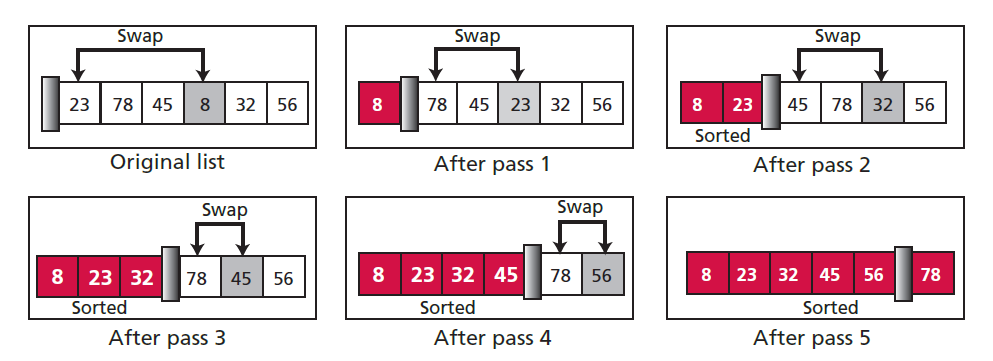
\includegraphics[width=0.9\textwidth]{\main/images/unit08/selection_sort_example.png}
					\end{center}
					\begin{sidenote}{Selection Sort Algorithm}
						\begin{lstlisting}
wall = leftmost
while (more passes)
  find smallest
  swap smallest and first
  wall++
						\end{lstlisting}
					\end{sidenote}
				\pagebreak
				\subsubsection{Bubble Sort}
					Move the smallest element from the unsorted list to after the separator. Move the separator one ahead.
					\begin{center}
						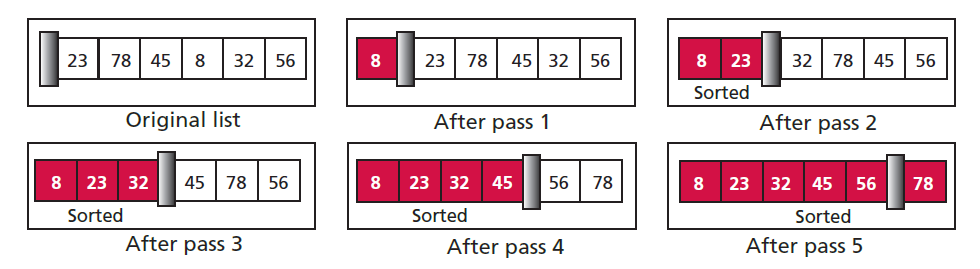
\includegraphics[width=0.9\textwidth]{\main/images/unit08/bubble_sort_example.png}
					\end{center}
					\begin{sidenote}{Bubble Sort Algorithm}
						\begin{lstlisting}
wall = leftmost
while (more passes)
  list[wall + 1] = smallest
  wall++
						\end{lstlisting}
					\end{sidenote}
				\subsubsection{Insertion Sort}
					Move the value after the separator to the correct place in the sorted list, and then move the separator one ahead.
					\begin{center}
						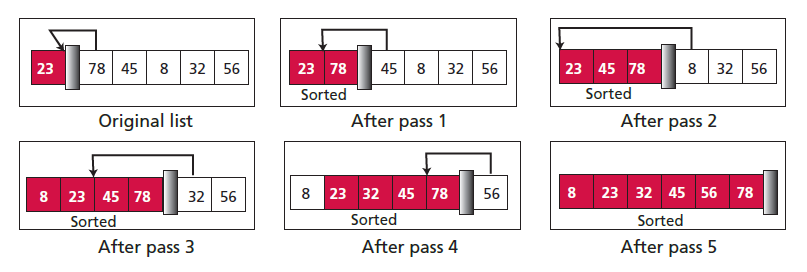
\includegraphics[width=0.9\textwidth]{\main/images/unit08/insertion_sort_example.png}
					\end{center}
					\begin{sidenote}{Insertion Sort Algorithm}
						\begin{lstlisting}
wall = leftmost
while (more passes)
  place current value in correct place
  wall++
						\end{lstlisting}
					\end{sidenote}
				\pagebreak
				\subsubsection{Other Sorting Algorithms}
					The three algorithms shown are the \emph{least efficient}. They form the foundation of more efficient algoirithms, such as
					\begin{itemize}[nosep]
						\item quicksort
						\item heap sort
						\item Shell sort
						\item bucket sort
						\item merge sort
						\item radix sort
						\item etc.
					\end{itemize}
			\subsection{Searching}
				\begin{definition}{Searching}
					The process of finding the location of a target among a list of objects. Two basic types: \concept{sequential search}, and \concept{binary search}.
				\end{definition}
				\subsubsection{Seqential Search}
					Can be used on any list -- does \emph{not} require the list to be sorted.

					Should only be used for small lists, or lists that are not searched often, as it is slow.

					Start searching for the target from the beginning of the list. Continue searching until either the target is found, or the end of the list is reached.

					\begin{center}
						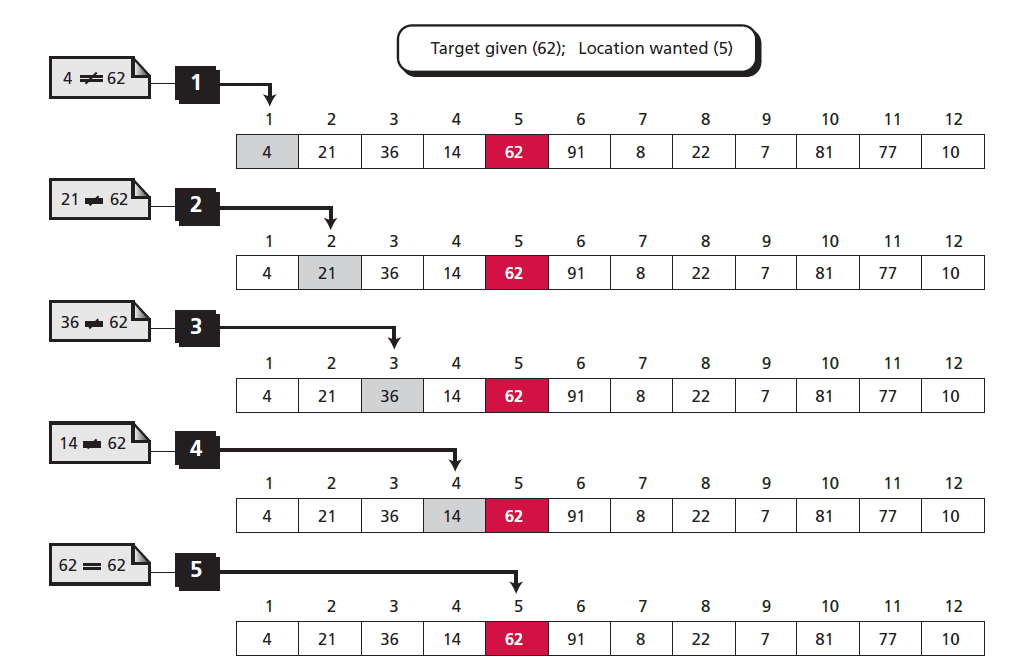
\includegraphics[width=0.9\textwidth]{\main/images/unit08/sequential_search.png}
					\end{center}
				\subsubsection{Binary Search}
					Used on sorted lists. Can be used efficiently on large lists.

					Check whether the target value is larger or smaller than the middle value. If the target value is smaller, only search the first half. If the target value is bigger, only search the second half.

					For whichever half is selected, compare to the middle value again, dividing the half into quarters. Continue doing so until the value is found, or it is determined that the value is not present. The value is not present if the value of \texttt{last} is smaller than the value of \texttt{first}.

					\begin{center}
						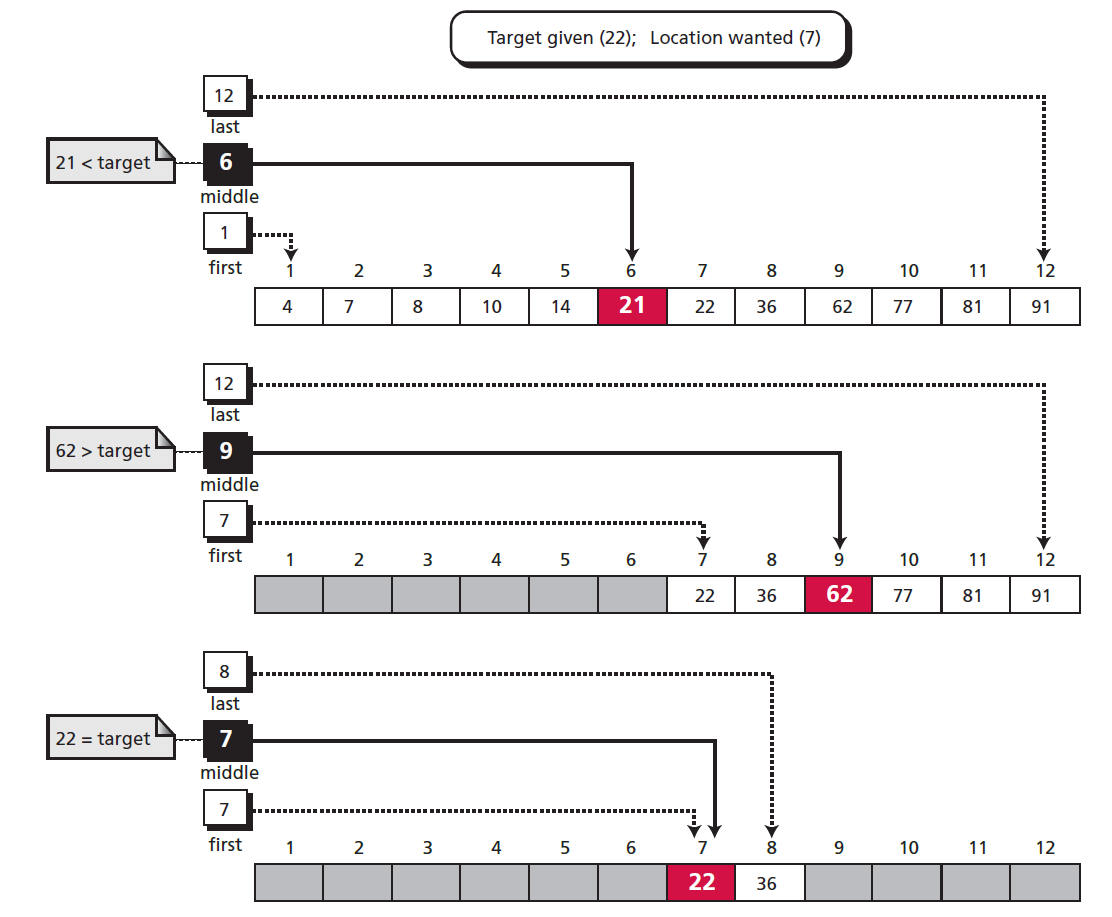
\includegraphics[width=0.9\textwidth]{\main/images/unit08/binary_search.png}
					\end{center}

					To determine the middle position, it is (first + last)/2. If the value is a fraction, ignore the fractional part.
		\pagebreak

		\section{Subalgorithms}
			\begin{definition}{Subalgorithm}
				A smaller algorithm that operates as a subunit of a larger algorithm.
			\end{definition}
			Advantages:
			\begin{itemize}
				\item Algorithms are more understandable
				\item A subalgorithm can be called many different times, without needing to be rewritten.
			\end{itemize}
			\begin{definition}{Structure Chart}
				A high-level design tool that shows the relationship betwen algorithms and subalgorithms. Used at the design level rather than the programming level.
			\end{definition}

	\rulechapterend

\end{document}